\section{Playtest second!}
Now that we have a passing test, we want to display some results as web pages.
The following examples utilize the Prado framework to display and manipulate
the database through SQLMap. Since SQLMap framework and Prado framework solve
different problems, they are both fairly independent, they can be used
together or separately.

\subsection{SQLMap and Prado}
To setup Prado, we need to create the follow files and directory structure
under our \tt{example/WebView} directory.
\begin{verbatim}
assets/                         % application public assets

protected/pages/Home.page       % default page
protected/pages/Home.php        % default page class
protected/runtime/              % run time data

protected/application.xml       % application configuration

index.php                       % application entry point
\end{verbatim}

The \tt{application.xml} and \tt{assets} directory are not necessary but we
will make use of them later. The \tt{application.xml} is used to define some
directory aliases and override the data source definitions in the
\tt{sqlmap.config}. This is because SQLite database files are defined
relatively, otherwise we don't need to override the data source definitions.
The example \tt{application.xml} is show in Example~\ref{example:2.0}.

\begin{example}\label{example:2.0}
Prado application.xml, defines path aliases and override SQLite database
location.
\begin{verbatim}
<?xml version="1.0" encoding="utf-8"?>
<application id="SQLMap Example" Mode="Debug">
  <paths>
    <alias id="Example" path="../../" />
    <using namespace="System.DataAccess.*" />
  </paths>
  <modules>
    <module id="SQLMap" class="TSQLMap"
            configFile="Example.sqlmap">
        <!-- override sqlmap.config's database provider -->
        <provider class="TAdodbProvider">
            <datasource driver="sqlite" host="../Data/test.db" />
        </provider>
    </module>
  </modules>
</application>
\end{verbatim}
\end{example}

The entry point to a Prado application in this example is \tt{index.php}.
Example~\ref{example:2.1} shows the basic \tt{index.php} content.
\begin{example}\label{example:2.1}
Prado application entry point, \tt{index.php}.
\begin{verbatim}
<?php
error_reporting(E_ALL);
require_once('/path/to/prado/framework/prado.php');
$application=new TApplication;
$application->run();
?>
\end{verbatim}
\end{example}

Now we are ready to setup a page to display our list of people.
Example~\ref{example:7} shows the Prado code for our display page. The key
piece is the TDataGrid.

\begin{example}\label{example:7}
Prado page for our Person list, \tt{Home.page}.
\begin{verbatim}
<!doctype html public "-//W3C//DTD XHTML 1.0 Strict//EN"
    "http://www.w3.org/TR/xhtml1/DTD/xhtml1-strict.dtd">
<html xmlns="http://www.w3.org/1999/xhtml" lang="en">
<head>
    <title>Person</title>
</head>
<body>
<com:TForm>
    <h1>Person List</h1>
    <com:TDataGrid id="personList">
        <com:TBoundColumn DataField="BirthDate"
                HeaderText="Birth Date"/>
    </com:TDataGrid>
</com:TForm>
</body>
</html>
\end{verbatim}
\end{example}

Of course, we still need to populate that TDataGrid. Example~\ref{example:8}
shows the PHP code for \tt{Home.php}. The operative method is \tt{loadData()}.
The rest is supporting code.

\begin{example}\label{example:8}
\tt{Home.php} class for our Person list page
\begin{verbatim}
<?php
Prado::using('Example.Models.Person');
class Home extends TPage
{
    private function loadData()
    {
        $sqlmap = $this->Application->getModule('SQLMap')->getClient();
        $this->personList->DataSource = $sqlmap->queryForList('SelectAll');
        $this->personList->dataBind();
    }

    public function onLoad($param)
    {
        if(!$this->IsPostBack)
            $this->loadData();
    }
}
?>
\end{verbatim}
\end{example}

If we run this now, we'll get a list like the one shown in
Figure~\ref{figure:2}.
\begin{figure}[!h]
    \centering
        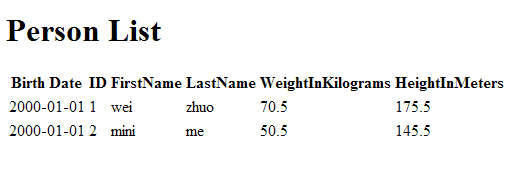
\includegraphics[width=0.75\textwidth]{grid1}
    \caption{A quick-and-dirty Person List}
    \label{figure:2}
\end{figure}
